% !Mode:: "TeX:UTF-8"
\chapter{Backend: Part II}
\begin{mdframed}  
	\textbf{Goal of Study}
	\begin{enumerate}[labelindent=0em,leftmargin=1.5em]
		\item Learn the principles of sliding window optimization; 
		\item Learn the basic knowledge about pose graph optimization.
		\item Pose graph optimization with g2o. 
	\end{enumerate}
\end{mdframed}

In the last lecture, we focused on graph optimization based on BA. BA can accurately optimize the pose and feature point position of each camera. However, in a larger scene, the high dimensionality of landmarks will seriously reduce the calculation efficiency, resulting in an increasing amount of calculation that cannot be real-time. The first part of this lecture will introduce a simplified, yet widely used optimization approach: pose graph.

\newpage
\section{Sliding Window Filter and Optimization}
\subsection{Controling the Structure of BA}

The graph optimization with camera pose and spatial points is called BA, which can effectively solve large-scale positioning and mapping problems. This is very useful in SfM, but in the real-time SLAM process, we often need to control the problem's scale to maintain real-time calculations. If the computing power is unlimited, we might calculate the entire BA every moment-but that does not meet the reality. The reality is that we must limit the calculation time of the back-end. For example, the BA scale cannot exceed 10,000 landmarks, the iterations cannot exceed 20 times, and the time used does not exceed 0.5 seconds, and so on. An algorithm that takes a week to reconstruct a city map like SfM is not necessarily effective in SLAM.

There are many ways to control the calculation scale, such as extracting keyframes from the continuous video \cite{Leutenegger2015}, only constructing the BA between the keyframe and the landmarks. The non-key frames are only used for localization and do not contribute to the mapping part. Even so, as time goes by, the number of keyframes will increase, and the scale of the map will continue to grow. For batch optimization methods like BA, the computational efficiency will (worryingly) continue to decline. To avoid this situation, we need to control the scale of the back-end problem. These methods can be theoretical or engineering.

For example, the simplest way to control the BA scale is to keep only the $N$ keyframes closest to the current moment and remove the earlier ones. Therefore, we will fix the BA within a time window, and those that leave this window will be discarded. This method is called the sliding window method \cite{Sibley2008}. Of course, we can change the criteria for selecting these $N$ keyframes. For example, it is unnecessary to take the closest in time, but according to a certain principle, take the keyframes that are close in time and expandable in space. To ensure that even when the camera is stopped, the BA structure will not shrink into a single point (this can easily lead to some bad degradation). If we think more deeply about the structure of frames and frames, we can also define a structure called ``covisibility graph'' like ORB-SLAM2 \cite{Mur-Artal2015} (see \autoref{fig:cov-graph}). The so-called co-visibility refers to those features that are observed together with the current keyframe). Therefore, in BA optimization, we take some keyframes and landmarks in the co-visibility graph to optimize. For example, we may pick about 20 co-visible keyframes with the current frame and leave the others unchanged. If we can construct the co-visibility relationship correctly, the optimization will remain optimal for a longer time.

\begin{figure}[!ht]
	\centering
	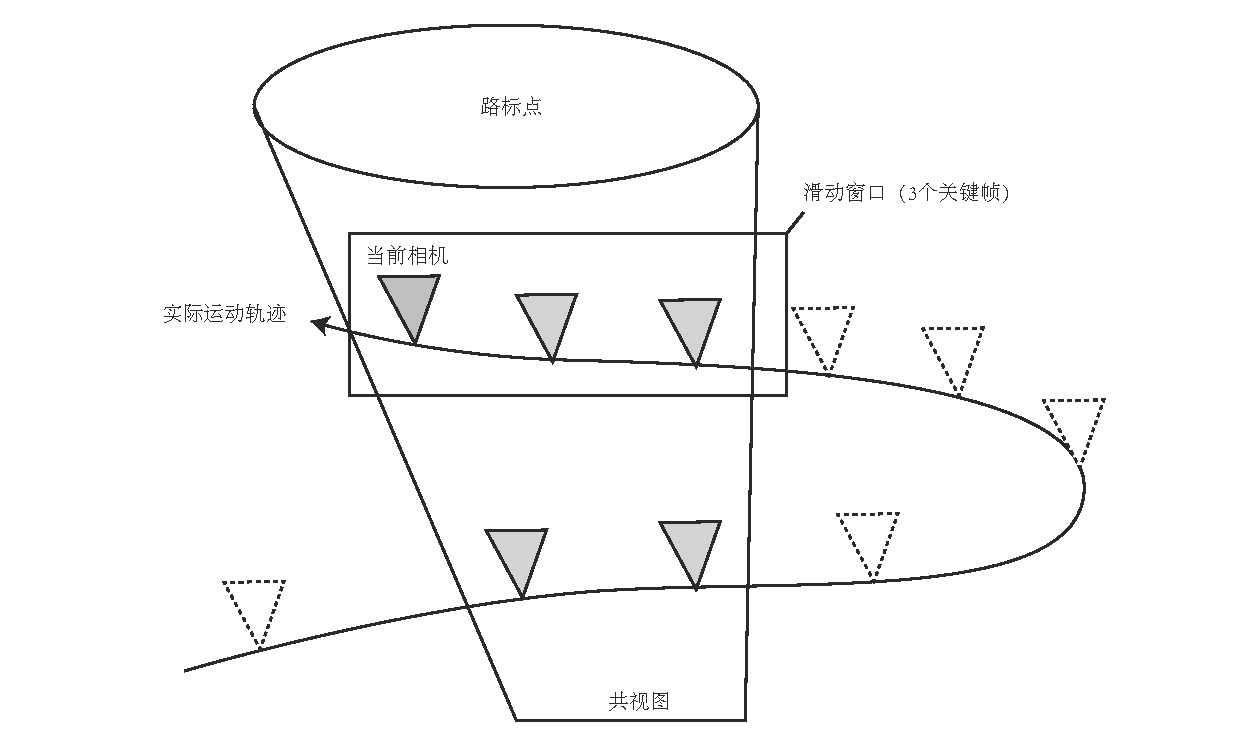
\includegraphics[width=0.8\textwidth]{backend2/cov-graph.pdf}
	\caption{Co-visibility graph in sliding window. }
	\label{fig:cov-graph}
\end{figure}

No matter whether it is a sliding window or a co-visibility approach, in general, it is a kind of engineering trade-off between full SLAM and real-time computing. But in theory, they also introduce a new problem: when we talk about "discarding" variables outside the sliding window or "fixing" variables outside the co-visibility graph, what is the specific operation of "discarding" and "fixing"? "Fixed" seems to be easy to understand. We only need to keep the keyframe estimates unchanged during optimization. But "discarding" refers to completely abandoning it, which means that the variables outside the window totally do not affect the variables in the window?  Or does the data outside the window should have some influence but is somehow ignored? 

Next, we will talk about these issues. How should they be dealt with in theory, and whether we can simplify them in engineering?

\subsection{Sliding Window}
Now consider a sliding window. Assume there are $N$ keyframes in this window, and their poses are denoted as $$\bm{x}_1, \ldots, \bm{x}_N,$$ we assume that they are in the vector space, that is, using Lie Algebra expression, then, what can we talk about these keyframes?

Obviously, we care about the location of these keyframes and their uncertainty. This corresponds to their mean and covariance under the assumption of Gaussian distribution. If these keyframes also correspond to a local map, we can also ask for the entire local map's mean and covariance. Suppose there are $M$ landmark points in this sliding window: $\bm{y}_1, \ldots, \bm{y}_N$, they form a local map together with the $N$ keyframes. Obviously, we can use the bundle adjustment method introduced in the last lecture to deal with this sliding window, including building a graph optimization model, building an overall Hessian matrix, and then marginalizing all landmarks to speed up the solution. After the marginalization, we get the conditional distribution of the poses, namely $$[\bm{x}_1, \ldots, \bm{x}_N | \bm{y}_1, \ldots, \bm{y}_M ] \sim N([\boldsymbol{\mu }_1, \ldots, \boldsymbol{\mu}_N]^\mathrm{T}, \boldsymbol{\Sigma}).$$ where $\boldsymbol{\mu}_k$ is mean of the $k$-th keyframe, $\boldsymbol{\Sigma}$ is the covariance matrix of all keyframes. So obviously, the mean part refers to the optimal result after BA, and $\boldsymbol{\Sigma}$ is the result of the marginalization, i.e., the matrix $\bm{S}$ mentioned in the previous lecture. We think that readers are already familiar with this process.

In a sliding window, another question is to ask, when the window moves, how should these state variables change? This matter can be discussed in two parts:

\begin{enumerate}
	\item We want to add a new keyframe into the window as well as its corresponding landmarks.
	\item We need to delete an old key frame in the window, and may also delete the landmarks it observes.
\end{enumerate}

At this time, the difference between the sliding window method and the traditional BA is revealed. If processed as a traditional BA, then this only corresponds to two BAs with different structures, and there is no difference in the solution. But in the case of sliding windows, we have to discuss these specific details.

\subsubsection{Adding New Keyframes}
Considering that the sliding window has established $N$ keyframes at the last moment, and we already know that they obey a certain Gaussian distribution, and their mean and variance are as described above. At this time, a new keyframe $\bm{x}_{N+1}$ has arrived, and the variables in the whole problem become a collection of $N+1$ keyframes and more road signs. In fact, this is still ordinary. We only need to follow the normal BA process. When all points are marginalized, the Gaussian distribution of these $N+1$ keyframe poses are obtained.

\subsubsection{Removing Old Keyframes}
When considering deleting old keyframes, a theoretical problem will emerge. For example, we want to delete the old keyframe $\bm{x}_1$. But $\bm{x}_1$ is not isolated. It will observe the same landmarks as other frames. After marginalizing $\bm{x}_1$, the whole problem will no longer be sparse. As in the previous lecture, let's take a schematic diagram, as shown in \autoref{fig:marg-frame}.

\begin{figure}[!ht]
	\centering
	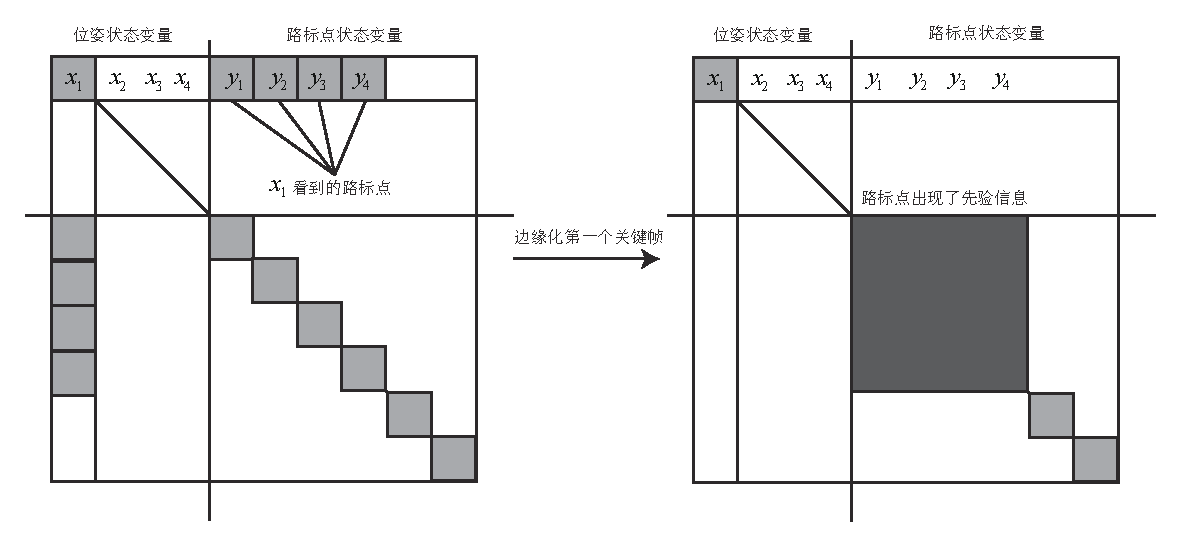
\includegraphics[width=1.0\textwidth]{backend2/marg-frame.pdf}
	\caption{Margining old keyframes will break the sparse structure of the Hessian.}
	\label{fig:marg-frame}
\end{figure}

In this example, we assume that $\bm{x}_1$ sees the landmarks from $\bm{y}_1$ to $\bm{y}_4$, so before processing, the Hessian matrix of the BA problem should be like the left side of this figure. There are non-zero blocks in the columns $\bm{y}_1$ to $\bm{y}_4$ in the $\bm{x}_1$ row, which means $\bm{x}_1 $ saw them. At this time, consider the marginalization $\bm{x}_1$. Please recall what we do in the Schur trick: We multiply the first row by the coefficient and adding it to the rows below the dividing line to eliminate the non-zero block in the first column; then use the first column to eliminate the non-zero block in the first row. But when we do this, the Hessian of the Landmark-Landmark part is filled with information by this operation, and it is no longer a diagonal block. This phenomenon is called (fill in) {\cite{Sibley2008}}.

Intuitively, fill-in means that when you ask for $P(\bm{x}_2, \bm{x}_3, \bm{x}_4, \bm{y}_1, \ldots \bm{y}_4|\bm{x}_1)$, because the marginalized keyframe sees some landmarks, these landmarks have one more constraint saying ``where they should be if $\bm{x}_1$ is set to the current value" (conditional distribution).Such a priori constraint describes the information about where these landmarks should be.

Recalling the marginalization mentioned in the previous lecture, when we marginalize the landmarks, the fill-in effect will appear in the pose block in the upper left corner. However, because BA does not require the pose block to be a diagonal block, the sparse BA solution is still feasible. However, when the keyframes are marginalized, it will destroy the diagonal block structure between the landmark points in the lower right corner. We cannot solve BA iteratively in the previous sparse method. This is obviously a terrible question. In fact, in the back end of the early EKF filter, people did maintain a dense Hessian matrix, which also made the back end of the EKF unable to handle higher dimension states.

However, if we make some modifications to the marginalization process, we can also maintain the sliding window BA's sparsity. For $\bm{y}_1$ to $\bm{y}_4$, they may fall into the three cases listed below:

\begin{enumerate}
	\item The landmark is only observed in $\bm{x}_1$ and does not appear in the remaining keyframes. Then you can just throw away the landmark without any impact on the window. This landmark is isolated.
	\item The landmark is seen in $\bm{x}_2$-$\bm{x}_4$, but will not be seen in the future. (This is just an assumption here, and it actually depends on the implementation of the frontend. Optical flow frontends like VINS \cite{Qin2018} or DSO will not track the missing feature points, so we can just assume this is the case.) Then you can also marginalize this landmark. When road signs are marginalized, a priori of the pose-pose part is generated, so it becomes the prior information of the future pose estimation.
	\item The landmark is seen in $\bm{x}_2$-$\bm{x}_4$ and may be seen in the future. Then this landmark should not be marginalized, because we will need to update its estimate later. In theory we can only maintain the dense structure in the landmark-landmark part, but in engineering, we can pretend that the observation of this landmark by $\bm{x}_1$ can be simply discarded (equivalent to thinking that $\bm{x}_1$ did not see it). So we kept the diagonal structure of the Landmark part at a small cost. In this case you don't have to do anything.	
\end{enumerate}


\subsubsection{Intuitive Explanation of the Marginalization in SWF}
We know that the meaning of marginalization in probability refers to decomposing a joint distribution into a conditional and marginal distribution. So intuitively speaking, when we marginalize a keyframe, we mean ``keep the current estimated value of this keyframe and find the conditional probability of other state variables conditioned on this keyframe.'' Therefore, when a keyframe is marginalized, the landmark points it observes will generate a priori information of ``\textbf{where these landmarks should be},'' which affects the estimated value of the rest. If these landmark points are then marginalized, their observers will get a priori information of ``\textbf{where the keyframe to observe them should be}.''

Mathematically, when we marginalize a certain keyframe, the description of the state variables in the entire window will change from a joint distribution to a conditional probability distribution. Taking the example above, it means:
\begin{equation}
	p\left( {{\bm{x}_1}, \ldots {\bm{x}_4},{\bm{y}_1}, \ldots {\bm{y}_6}} \right) = p\left( {{\bm{x}_2}, \ldots ,{\bm{x}_4},{\bm{y}_1}, \ldots {\bm{y}_6}|{\bm{x}_1}} \right)\underbrace {p\left( {{\bm{x}_1}} \right)}_{\text{discarded}}.
\end{equation}
Then discard the marginalized part of the information. After the variable is marginalized, we should no longer use it in engineering. Therefore, the sliding window method is more suitable for VO systems but not for large-scale mapping systems.

Since g2o and Ceres have not explicitly supported the marginal operation in the sliding window method \footnote{In the project, we can walk around g2o and Ceres's restrictions through some clever tricks, but this is often very troublesome and not suitable for demos. }, we omit the corresponding experimental part in this section. I hope the theoretical part can help readers understand some SLAM systems based on sliding windows.

\section{Pose Graph Optimization}
\subsection{Definition of Pose Graph}

